\setchapterpreamble[u]{\margintoc}

\chapter{Espacios CW-complejos} \label{CW}
\section{Espacio de adjunción}
\begin{definition}
Sean $X,Y$ espacios topológicos, $A \subset X$ un subespacio cerrado y
$f\colon A \to Y$ una aplicación continua. Dados $x \in X$, $y \in Y$,
escribiremos $x \sim y$ si $x \in A$ e $y=f(x)$. Se define el
\textbf{espacio de adjunción} o \textbf{de pegamiento} como
\[X \cup_f Y:=\frac{X\sqcup Y}{\sim}\]
Decimos que $f$ es la \textbf{aplicación de adjunción} o de
\textbf{pegamiento} de $X\cup_fY$.
\end{definition}

Si $Y=\{\star\}$, $f=\text{Cte}_\star$, por lo que $x\sim z$ para todos $x,z
\in A$ y $X\cup_f Y=X/A$.

\begin{lemma}
La proyección canónica $p\colon X \sqcup Y \to X\cup_f Y$ verifica las
siguientes condiciones:
\begin{enumerate}
\item $p(Y)$ es cerrado;
\item $p|_Y$ es un homeomorfismo sobre su imagen;
\item $p(X\backslash A)$ es abierto;
\item $p|_{X\backslash A}$ es un homeomorfismo sobre su imagen.
\end{enumerate}
Como consecuencia, podemos considerar a $Y$ y $X\backslash A$ como subespacios
de $X\cup_f Y$.
\end{lemma}

\marginnote[-2.2cm]{
\begin{kaobox}[frametitle=Aplicaciones abiertas y cerradas]
Una aplicación $f\colon X \to Y$ es abierta (resp. cerrada) si la imagen de
un abierto (resp. cerrado) en $X$ es abierto (resp. cerrado) en $Y$. Si $f$ es
biyectiva, su inversa será continua si y sólo si $f$ es abierta o cerrada.

Un ejemplo de aplicación abierta (y cerrada) son las proyecciones.
\end{kaobox}
}

\begin{proof}
Como $X\sqcup Y$ es una unión disjunta de espacios topológicos, $Y$ es un
subespacio cerrado de $X\sqcup Y$. Además, $A$ es cerrado en $X$ si y sólo si
lo es en $X \sqcup Y$, por lo que $A\cup Y$ es cerrado en $X \sqcup Y$. Pero
$A\cup Y=p^{-1}[p(Y)]$, por lo que $p(Y)$ es cerrado.

Pasemos al segundo ítem: para ver que $p|_Y$ es un homeomorfismo sobre su
imagen, necesitamos ver que es cerrada e inyectiva.

Sea $y\in Y$: si $y \not\in f(A)$, se tiene de forma trivial que $p^{-1}([y])=
\{y\}$. Si $y \in f(A)$, podemos hallar un $x \in A$ tal que $f(x)=y$.

Como $x \in A \subseteq X$, podemos hallar un $y' \in X\sqcup Y$ tal que $y
\sim y'$. Si $y' \in Y$, $y=f(x)=y'$ y no hay nada que probar. Si asumimos que
$y'\neq y$, $y \in X$. Teniendo en cuenta que 
\[(p|_Y)^{-1}([y])=p^{-1}([y])\cap Y\]
se sigue que $y' \not \in (p|_Y)^{-1}([y])$, por lo que $p|_Y$ es inyectiva.

Para ver que $p|_Y$ es cerrada, sea $C$ un subespacio cerrado de $Y$. Como
$p(Y)$ es cerrado en $X \cup_f Y$, $p(C)$ es cerrado en $p(Y)$ si y sólo si lo
es en $X \cup_f Y$. Ésto es tanto como decir que $p^{-1}[p(C)]$ es cerrado en
$X \sqcup Y$.

Observamos que
\[p^{-1}[p(C)]=f^{-1}(C)\sqcup C\]
por lo que $p^{-1}[p(C)]$ es una unión de cerrados. En consecuencia, $p(C)$ es
cerrado en $p(Y)$, de donde se sigue que $p|_Y$ es una aplicación cerrada.
Ésto concluye el segundo ítem.

Como $A$ es cerrado en $X$, $X\backslash A$ es abierto en $X \sqcup Y$. Dado
que\\ $p^{-1}[p(X\backslash A)]=X\backslash A$, se sigue que
$p(X\backslash A)$ es abierto en $X\cup_f Y$.

Pasemos al último item: dado un $x \in X\backslash A$, $p^{-1}([x])=\{x\}$,
por lo que $p|_{X\backslash A}$ es inyectivo. Dado que $p$ es continua, sólo
necesitamos ver que es abierta para deducir la tesis.

Sea $U\subseteq X\backslash A$: como $p(X\backslash A)$ es abierto en
$X\cup_f Y$, $p(U)$ será abierto en $p(X\backslash A)$ si y sólo si lo es en
el espacio de adjunción, o equivalentemente, $p^{-1}[p(U)]$ es abierto en
$X\sqcup Y$.

Dado que $U\subseteq X\backslash A$, se tiene que $U=p^{-1}[p(U)]$. Si $U$
es abierto de $X\backslash A$ también lo será de $X\sqcup Y$, por lo que
$p(U)$ es abierto en el espacio de adjunción. Ésto concluye la demostración.
\end{proof}

\marginnote[-2.2cm]{
\begin{kaobox}[frametitle=Primer axioma de numerabilidad]
Un espacio topológico $X$ verifica el primer axioma de numerabilidad (1AN)
si, dado $p \in X$, existe una base de entornos numberable de $X$.

Una base de entornos de $p$ es una familia de entornos $\{V_\alpha\colon
\alpha \in A\}$ tal que, dado un entorno $U \subseteq X$ de $p$, $U$
contiene al menos a un $V_\alpha$.
\end{kaobox}
}

\begin{lemma}
\label{AdjC2} Sean $X$, $Y$ espacios de tipo $C_2$. Si $X$ e $Y$ son 1AN,
$X\cup_f Y$ es de tipo $C_2$.
\end{lemma}

\begin{proof}
El espacio $X\cup_f Y$ es compacto por ser imagen de un espacio compacto
(en este caso $X\sqcup Y$) por una aplicación continua (la proyección
canónica $p\colon X\sqcup Y \to X\cup_f Y$).

Queremos ver que $X\cup_f Y$ es $T_2$. Dado que $X\cup_f Y$ es un espacio
cociente y $X$, $Y$ son $T_2$, basta ver que el conjunto
\[\{(x,y) \in (X\cup_f Y)^2\colon y=f(x)\}=G(f)\]
es cerrado. Dado que $X$ e $Y$ son 1AN, $(X\sqcup Y)^2$ es 1AN, por lo que
$G(f)$ será cerrado si y sólo si contiene a todos sus puntos de acumulación.

\marginnote[-2.2cm]{
\begin{kaobox}[frametitle=La propiedad de Hausdorff en los cocientes]
Sea $W$ un espacio de Hausdorff y $\sim$ una relación de equivalencia sobre
los puntos de $W$. Si el conjunto
\[\{(x,y) \in W^2: x\sim y\}\]
es cerrado en $W^2$, $W/\sim$ es un espacio de Hausdorff.
\end{kaobox}
}

Sea $(z_n)$ una sucesión de $G(f)$. Por compacidad de $X \sqcup Y$, existe
una subsucesión $(z_{n_k})$ convergente a un cierto $z_0 \in X\sqcup Y$. Por
definición de $G(f)$, existe una sucesión $(x_k)$ de $A$ tal que
\[z_{n_k}=(x_k,f(x_k))\]
Se tiene entonces que $(x_k)$ converge a $x_0$, que está en $A$ por ser
cerrado de $X$. Además, como $f$ es continua, $f(x_k)$ converge a $f(x_0)$.

De esta forma, $(z_{n_k})$ converge a $(x_0,f(x_0)) \in G(f)$. Dado que
$X\sqcup Y$ es $T_2$, $z_0=(x_0,f(x_0))$, por lo que $z_0 \in G(f)$. De aquí
se sigue que $G(f)$ es cerrado. Por tanto, $X\cup_f Y$ es $T_2$.
\end{proof}

\begin{lemma}\lablemma{RepAdj}
Sean $X$, $Y$, $W$ espacios $C_2$, $A \subset X$ un subconjunto cerrado y
$g\colon X\sqcup Y \to W$ una aplicación continua y sobreyectiva. Supongamos
que, para todo punto $w \in W$, se cumple que
\[g^{-1}(w)=\left\{
\begin{array}{c}
\text{un único punto de $X\backslash A$}\\
\lor\\
\text{$\{y\}\cup f^{-1}(y)$ para algún $y \in Y$}
\end{array}
\right.\]
Entonces, $g$ induce un homeomorfismo entre $W$ y $X \cup_f Y$.
\end{lemma}

\begin{proof}
Sea $\p\colon X\sqcup Y \to X \cup_f Y$ la proyección canónica. Se define la
aplicación
\begin{diag}
\overline g\colon X\cup_f Y \arrow[r]& W\\[-8mm]
\left[x\right] \arrow[maps to, r] & g(x)
\end{diag}

\marginnote[-2.2cm]{
\begin{kaobox}[frametitle=Continuidad de la inversa]
Si $f\colon X \longrightarrow Y$ es una biyección continua, donde $X$ es
compacto e $Y$ es de Hausdorff, $f$ es un homeomorfismo.
\end{kaobox}
}

Supongamos que $\overline g$ está bien definida y es una biyección continua:
por el \reflemma{AdjC2}, tenemos que $X\cup_f Y$ es de tipo $C_2$. Como $W$ es
$T_2$, se sigue que $\overline g$ tiene inversa continua, por lo que es un
homeomorfismo y el lema queda probado.

Empecemos por ver que $\overline{g}$ está bien definida: sean $x_1, x_2 \in
A$ elementos asociados y diferentes. Existirá un $y \in f(A)$ tal que $f(x_1)=
y=f(x_2)$. Si $w=g(x_1)$, se tiene por hipótesis que
\[g^{-1}(w)=\{y\}\cup f^{-1}(y) \implies g(x_1)=w=g(x_2)\]
Si $x \in X\backslash A$, $x$ sólo está asociado consigo mismo, de forma que
$\overline{g}$ está trivialmente bien definida. Dado que todas las
antiimágenes por $g$ de un cierto $w \in W$ están asociadas, $\overline{g}$ es
también inyectiva.

Veamos que $\overline{g}$ es continua: si $C \subseteq W$ es cerrado,
$g^{-1}(C)$ es cerrado en $X\sqcup Y$, por lo que $\pi^{-1}[g^{-1}(C)]$ es
cerrado en $X\cup_f Y$. Notar que
\[\pi^{-1}[g^{-1}(C)]=\overline{g}^{-1}(C)\]
por lo que se sigue la continuidad de $\overline{g}$.
\end{proof}

Sea $g\colon X \to W$ una aplicación continua y sobreyectiva entre espacios de
tipo $C_2$. Supongamos que existe un $w_0 \in W$ de forma que $A=g^{-1}(w_0)$
es un cerrado en $X$ y $g^{-1}(w)$ es un único punto de $X\backslash A$ para
todo $w\neq w_0$.

Si $\{\star\}$ es el espacio puntual, la aplicación constante
$f\colon A \to \{\star\}$ es continua, y se verifica que $X \cup_f \{\star\}$
es homeomorfo a $X/A$. Por el \reflemma{RepAdj}, se tiene que
\[W \cong X \cup_f \{\star\}\cong X/A\]

%Un espacio topológico Hausdorff y 2AN $X$ es una $n$-variedad si, dado $p \in
%$X$, existe un entorno abierto $U \subseteq X$ de $p$ homeomorfo a una bola
%abierta de $\mb{R}^n$. Éstos homeomorfismos se denominan cartas o
%parametrizaciones locales de $X$.

\begin{example} \label{Sn_CW}
Sea $h\colon D^n\backslash S^{n-1} \to \mb{R}^n$ un homeomorfismo, $\mc{N}=
(0,0,\dots,0,1)$ y $S^n_+=S^n\backslash\mc{N}$. La \textbf{proyección
estereográfica}, dada por
\begin{diag}
\Phi\colon S^n_+ \arrow[r] & \mb{R}^n\\[-8mm]
(x_1,\dots,x_{n+1}) \arrow[maps to, r] &
	\displaystyle\left(\frac{x_1}{1-x_{n+1}},\dots,\frac{x_n}{1-x_{n+1}}\right)
\end{diag}
es un homeomorfismo. Una posible parametrización de $h$ es
\[h(z)=\frac{z}{1-\|z\|}\]
Se define la aplicación $g\colon D^n \to S^n$ dada por
\[g(x)=\begin{cases}
\mc{N} &\text{ si $x \in S^{n-1}$}\\
(\Phi^{-1}\circ h)(x) &\text{ si $x \in D^n\backslash S^{n-1}$}
\end{cases}\]
Se tiene entonces que $g$ es continua y sobreyectiva por construcción.

Como $\mc{N} \in S^{n-1}$, $g^{-1}(\mc{N})=\{\mc{N}\}$ es un cerrado en $D^n$.
Dado que $\Phi$ y $h$ son aplicaciones biyectivas, $g^{-1}(z)$ es un único
punto para todo $z\neq \mc{N}$. Aplicando el lema \reflemma{RepAdj}, se tiene
entonces que
\[S^n\cong \frac{D^n}{S^{n-1}}\]
que es la adjunción de $D^n$ a un espacio puntual.
\end{example}

\begin{marginfigure}
\resizebox{\textwidth}{!}{
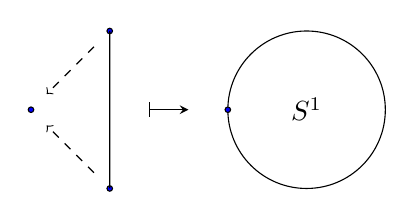
\begin{tikzpicture}
\draw[fill=blue] (0,0) circle (1pt);

\draw[dashed, -to] (.8,.8) -- (.2,.2);
\draw[dashed, -to] (.8,-.8) -- (.2,-.2);

\draw[fill=blue] (1,1) circle (1pt) -- (1,-1) circle (1pt);

\draw[|-stealth] (1.5,0) -- (2,0);

\draw (3.5,0) node {$S^1$} circle (1cm);
\draw[fill=blue] (2.5,0) circle (1pt);
\end{tikzpicture}
}
\caption{\labfig{CWS1} Conjunto $S^1$ construido como espacio de adjunción.}
\end{marginfigure}
\begin{marginfigure}
\resizebox{\textwidth}{!}{
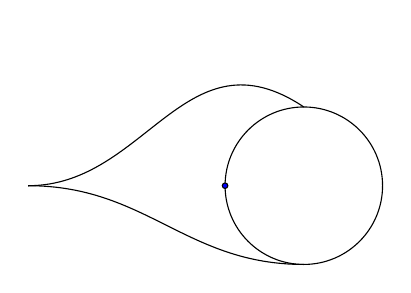
\begin{tikzpicture}
\draw (3.5,0) circle (1cm);
\draw[fill=blue] (2.5,0) circle (1pt);

\draw (3.5,-1) .. controls (2,-1) and (1.5,0) .. (0,0);
\draw (3.5,1) .. controls (2,2) and (1.5,0) .. (0,0);
\end{tikzpicture}
}
\caption[Espacio $S^1$ con dos segmentos adicionales, creando una figura
ocho.]{Podemos adjuntar nuevas células a las células preexistentes para
recrear espacios más complejos.}
\end{marginfigure}


\subsection{Células y adjunción}
Supongamos que $X=D^n$ para algún $n > 0$ y $A=S^{n-1}=\p D^n$. Decimos que el
espacio
\[Y_f:=D^n\cup_f Y\]
es la \textbf{adjunción de una $n$-célula} al espacio $Y$.

\begin{example}\labexample{Sn_CW}
En la figura \reffig{CWS1}, vemos cómo $S^1\cong \{\star\}_f$, siendo
$f\colon \p D^1=\{0,1\}\to \{\star\}$ la aplicación constante. En general,
$S^n$ se puede obtener como $\{\star\}_{f_n}$, siendo $f_n\colon \p D^n \to
\{\star\}$.
\end{example}

\begin{lemma}\lablemma{EntornoCompacto}
Sea $f: S^{n-1} \to Y$ una aplicación continua. Si $Y$ es un espacio $C_2$,
existe un entorno compacto $U_f$ de $Y$ en $Y_f$ tal que $Y$ es un retracto
por deformación fuerte de $U_f$.
\end{lemma}

\begin{proof}
Sea $U=\{x \in D^n: \|x\| \geq 1/2\}$. El cerrado $U$ es un entorno compacto
de $S^{n-1}$ en $D^n$. Definimos la homotopía $F\colon (U \sqcup Y)\times I
\to U\sqcup Y$ como
\[F(x,t)=
\begin{cases}
x &\text{ si }x \in Y \\
\displaystyle
(1-t)x+t\frac{x}{\|x\|} &\text{ si }x \in U
\end{cases}\]

Tenemos que $F$ es una aplicación continua que verifica las siguientes
propiedades:
\begin{enumerate}
\item $F(x,0)=x$ para todo $x \in U\sqcup Y$.
\item $F(x,1) \in S^{n-1}\sqcup Y$ para todo $x \in U \sqcup Y$.
\item $F(x,t)=x$ para todo $x \in S^{n-1}\sqcup Y$ y todo $t \in I$.
\end{enumerate}
Se sigue que $S^{n-1}\sqcup Y$ es un retracto por deformación fuerte de
$U\sqcup Y$.

Si $p\colon D^n \sqcup Y \to Y_f$ denota a la proyección canónica, se define
$U_f$ como la imagen de $U$ mediante $p$. Queremos ver que $Y$ es un retracto
por deformación fuerte de $U_f$ en $Y_f$. Para ello, considérese la
homotopía
\begin{diag}
G\colon U_f\times I \arrow[r] & U_f\\[-8mm]
(\left[x\right],t)\arrow[maps to,r] & F(x,t)
\end{diag}

Es fácil ver que $G$ está bien definida. Para ver que es continua, considérese
el diagrama conmutativo
\begin{diag}
(U\sqcup Y)\times I \arrow{r}{F} \arrow{d}{p\times \id_I}&
	U\sqcup Y \arrow{d}{p}\\
U_f\times I \arrow{r}{G} & U_f
\end{diag}

Dado que $F$ y $p$ son continuas, $G\times (p\times \id_I)=p\circ F$ es
continua, por lo que $G$ es continua. De aquí se sigue que $Y$ es un retracto
por deformación fuerte de $U_f$.
\end{proof}

\begin{proposition}
Dada una aplicación continua $f\colon S^{n-1} \to Y$,
\[H_p(Y_f,Y)\cong
\begin{cases}
\mb{Z} & \text{ si $p=n$}\\
0 & \text{ si no}
\end{cases}\]
\end{proposition}

\begin{proof}
Consideremos la composición
\[h\colon D^n \hookrightarrow D^n\sqcup Y \xrightarrow{p} Y_f\] 
El espacio $D^n\backslash S^{n-1}$ es homeomorfo a $Y_f\backslash Y$, puesto
que $Y_f=Y\cup_f D^n$, de forma que $h$ induce un homeomorfismo relativo entre
los pares $(D^n,S^{n-1})$ e $(Y_f,Y)$.

La esfera $S^{n-1}$ es un retracto por deformación fuerte del entorno compacto
$U=\{x \in D^n: \|x\| \geq 1/2\}$, y sabemos por el
\reflemma{EntornoCompacto} que $Y$ es un retracto por deformación fuerte de
algún entorno $U_f$ compacto de $Y$ en $Y_f$. Por el teorema del homeomorfismo
relativo (\refthm{HomeoRelativo}), se tiene que
\[h_*\colon H_*(D^n,S^{n-1}) \longrightarrow H_*(Y_f,Y)\]
es un isomorfismo.

Se tiene entonces que
\[H_*(Y_f,Y) \cong H_*(D^n,S^{n-1}) \cong \tilde{H}_*(S^n)\cong
\begin{cases}
\mb{Z} & \text{ si }p=n \\
0 & \text{ si no}
\end{cases}\]
\end{proof}

\begin{proposition} \labprop{HomoCW}
Sea $Y$ un espacio topológico y $f\colon S^{n-1} \to Y$ una aplicación
continua. Si $f_*\colon \tilde{H}_{n-1}(S^{n-1}) \to H_{n-1}(Y)$,
\begin{enumerate}
\item $H_p(Y_f)\cong H_p(Y)$ para todo $p$ distinto a $n$ y $n-1$;
\item $H_{n-1}(Y_f)\cong H_{n-1}(Y)/\im f_*$;
\item la sucesión
\begin{diag}
0 \arrow[r]& H_n(Y) \arrow[r]& H_n(Y_f) \arrow[r]&
\ker f_* \arrow[r]& 0
\end{diag}
es exacta.
\end{enumerate}
\end{proposition}

\begin{proof}
Consideremos la sucesión exacta larga asociada al par de espacios $(Y_f,Y)$:
\[\dots \longrightarrow H_{p+1}(Y_f,Y) \longrightarrow H_p(Y)
\xrightarrow{\beta} H_p(Y_f) \longrightarrow H_p(Y_f,Y) \longrightarrow \dots\]
Como vimos en el \refexample{Sn_CW},
\[H_p(Y_f,Y)\cong \tilde{H}_p(S^n) \cong \tilde{H}_{p-1}(S^{n-1})\]

Para $p\neq n,n-1$, $\tilde{H}_p(S^n)=0$, por lo que $\ker
\beta=0$ y $\im \beta=H_p(Y_f)$. Se sigue entonces la primera afirmación:
\[H_p(Y_f) \cong H_p(Y)\]

Para $p=n$ y $p=n-1$, se tiene la sucesión exacta
\begin{align*}
0=\tilde{H}_n(S^{n-1}) &\longrightarrow H_n(Y) \longrightarrow H_n(Y_f)
\xrightarrow{\beta} \tilde{H}_{n-1}(S^{n-1}) \xrightarrow{f_*} \\
&\xrightarrow{f_*} H_{n-1}(Y) \xrightarrow{\alpha} H_{n-1}(Y_f)
\longrightarrow \tilde{H}_{n-2}(S^{n-1})=0
\end{align*}
donde $\im \beta=\ker f_*$, $\im f_*=\ker \alpha$ y $\im \alpha=H_{n-1}(Y_f)$
por exactitud. Aplicando el primer teorema de isomorfia, se tiene la segunda
afirmación:
\[H_{n-1}(Y_f)=\im \alpha \cong \frac{H_{n-1}(Y)}{\ker \alpha}=
\frac{H_{n-1}(Y)}{\im f_*}\]

Ahora bien: como $\im \beta=\ker f_*$, la sucesión
\[0 \longrightarrow H_n(Y) \longrightarrow H_n(Y_f) \xrightarrow{\beta}
\ker f_* \longrightarrow 0\] es exacta, que es la tercera afirmación.
\end{proof}

\section{Espacios CW-complejos}
Sean $D_1^n,\dots, D_p^n$ una familia de $n$-células disjuntas con respectivas
fronteras $S^{n-1}_1,\dots,S^{n-1}_p$. Dado un $1 \leq i \leq p$, considérese
la aplicación continua
\[f_i\colon S^{n-1}_i \longrightarrow Y\]
siendo $Y$ un espacio topológico arbitrario. Si $\mc{D}^n=D^n_1\sqcup\dots
\sqcup D^n_p$ y $\mc{S}^{n-1}=\p \mc{D}^n=S^{n-1}_1\sqcup \dots S^{n-1}_p$,
definimos sobre $\mc{D}^n\sqcup Y$ la siguiente relación de equivalencia:
\[\forall x \in S^{n-1}_i \quad x \sim f_i(x); \quad i=1,\dots,p\]
Definimos entonces el espacio
\[Y_{f_1,\dots,f_p}=\frac{\mc{D}^n\sqcup Y}{\sim}\]

\begin{proposition}
Sea $(X,Y)$ un par de espacios $C_2$. Si existe un homeomorfismo relativo
\[F\colon (\mc{D}^n,\mc{S}^{n-1})\longrightarrow(X,Y)\]
que sea una prolongación continua de $f_1,\dots,f_p$, entonces $X$ es
homeomorfo a $Y_{f_1,\dots,f_p}$.
\end{proposition}

\begin{marginfigure}
\centering
\begin{subfigure}[b]{\textwidth}
\resizebox{\textwidth}{!}{
\begin{tikzpicture}

\draw[fill=green] (0,2) circle (1pt) -- (1.4,2) circle (1pt);
\draw[dashed, -stealth] (.1,2-1/7) -- (.6,2-6/7);

\draw[fill=green] (.7,1) circle (1pt);

\draw[dashed, -stealth] (.1,1/7) -- (.6,6/7);
\draw[dashed, -stealth] (1.3,2-13/7) -- (.8,2-8/7);

\draw[fill=green] (0,0) circle (1pt) -- (1.4,0) circle (1pt);

\draw[|-stealth] (1.5,1) -- (3,1);

\draw (4,1) circle (.7cm);
\draw[fill=green] (4,1.7) circle (1pt) -- (4,2.7) circle (1pt);

\end{tikzpicture}
}
\caption{Usando $1$-células, podemos construir un complejo de dimensión
$1$...}
\end{subfigure}
\begin{subfigure}[b]{\textwidth}
\resizebox{\textwidth}{!}{
\begin{tikzpicture}
\draw (0,0) circle (.7cm);
\draw[fill=green] (0,.7) circle (1pt) -- (0,1.7) circle (1pt);

\draw[|-stealth] (1.2,0) -- (2,0);

\draw[pattern=north west lines, pattern color=blue]
	(3,0) circle (.7cm) node {\contour{white}{$D^2$}};
\draw[fill=green] (3,.7) circle (1pt) -- (3,1.7) circle (1pt);


\end{tikzpicture}
}
\caption{...y después añadir células de orden superior, creando figuras más
complejas como una piruleta.}
\end{subfigure}
\end{marginfigure}

\begin{definition}
\begin{enumerate}
\item Un \textbf{CW-complejo finito de dimensión 0} es una colección finita de
puntos $\{p_1,\dots,p_n\} \subset \mb{R}^t$.
\item Sea $Y$ un CW-complejo finito de dimensión $k \geq 0$. Un espacio
topológico $C_2$ $X$ es un \textbf{CW-complejo finito de dimensión $n$} si
existen $f_i\colon S^{n-1} \longrightarrow Y$, $i=1,\dots,s$, tales que $X$ es
homeomorfo a $Y_{f_1,\dots,f_s}$.
\end{enumerate}
\end{definition}

Hemos definido los CW-complejos de dimensión $n$ como un proceso iterativo que
da lugar a una serie de CW-complejos intermedios
\[X^0 \subseteq X^1 \subseteq \dots \subseteq X^n\]
Cada uno de los $X^k$ se denomina \textbf{$k$-esqueleto} del CW-complejo. Notar
que $X^n$ es el CW-complejo completo.

\begin{example}\labexample{S2CW}
El \refexample{Sn_CW} describe una construcción de $S^2$ como CW-complejo de
forma que el 1-esqueleto y el 0-esqueleto son el mismo conjunto, porque no
adjuntamos ninguna 1-célula a $X^0$. Pero un CW-complejo puede admitir muchas
estructuras diferentes. 

Consideremos la siguiente estructura: sean
\[X^0=\{(1,0,0), (0,1,0),(-1,0,0)\}\]
tres puntos del ecuador. Adjuntamos a $X^0$ tres 1-células, $D^1_1$, $D^1_2$
y $D^1_3$, de forma que $S^1\cong X^1$.

Finalmente, adjuntamos dos 2-células $D^2_1$ y $D^2_2$ a $X^1$. Esto sería
$X^2$, que es homeomorfo a todo $S^2$.

En general, podemos generar una descomposición de $S^n$ de forma que cada
$k$-esqueleto sea $S^k$ ($k=0,1,2,\dots,n$); no obstante, en ese caso
tendríamos que el 0-esqueleto son dos puntos, dado que
\[S^0=\{x \in D^1: \|x\|=1\}=\{x \in [-1,1]: |x|=1\}=\{\pm 1\}\]
\end{example}

\begin{marginfigure}
\includegraphics{Figures/S2CW.pdf}
\caption{Espacio $S^2$ construido utilizando el \refexample{S2CW}.}
\end{marginfigure}

De esta forma, tenemos que un espacio topológico no induce una descomposición
como CW-complejo de forma única. Si comparamos este proceso con el que
seguimos en el \refexample{Sn_CW}, tenemos que no tienen el mismo número de
células y sus $1$-esqueletos no son homeomorfos, de forma que no son
\textit{estructuras equivalentes}.

\begin{theorem}[Caracterización de CW-complejos finitos]\labthm{TCCWF}
Un espacio topológico compacto $X$ es un CW-complejo finito de dimensión $n$
si y sólo si podemos hallar una sucesión de subespacios
\[X^0 \subseteq X^1 \subseteq \dots \subseteq X^n=X\]
y una partición de subconjuntos
\[\{D_i^k:\; k=0,1,\dots,n; \;i=1,2,\dots,r_k\}\]
(llamada \textbf{descomposición celular}) tales que
\begin{enumerate}
\item existe un homeomorfismo relativo
\[h\colon (D^k,S^{k-1}) \to
(\overline{D^k_i},\overline{D^k_i}\backslash D^k_i)\]
para cada $i$ y $k$;
\item dado un $1 \leq k \leq n$, $\overline{D^k_i}\backslash D^k_i
\subseteq X^{k-1}$.
\end{enumerate}
\end{theorem}

Hagamos un par de incisos en este teorema.

\begin{itemize}
\item Observar que $\overline{D^k_i}\backslash(\overline{D^k_i}\backslash
D^k_i)=D^k_i$. Aplicando el teorema anterior, se sigue que $D^k_i$ es
homeomorfo a una bola abierta de $\mb{R}^k$. Esto implica que las $n$-células
son conexas, compactas y abiertas para todo $n > 0$.
\item La condición de compacidad viene dada porque la adjunción de espacios
compactos es compacto, pero ninguna de las otras condiciones garantizan que
$X$ sea compacto.
\end{itemize}

\begin{example}
\begin{enumerate}
\item Este teorema proporciona otra forma de ver que $S^n$ admite una
estructura de CW-complejo: para $n=1$, sea $f\colon [0,2\pi] \to \mb{R}^2$ la
aplicación $f(t)=(\cos t,\sin t)$. Tenemos que $X=S^1$ admite una estructura
de CW-complejo tomando
\begin{align*}
X^0&=\{(1,0)\}; 	& X^1&=S^1;\\
D^0&=\{(1,0)\}; 	& D^1&=f(]0,1[]);
\end{align*}
Para $n=2$, sea $g\colon [0,1]\times [0,1] \to \mb{R}^3$ la aplicación
\[g(u,v)=(\cos(2\pi u)\cos(2\pi v),\cos(2\pi u)\sin(2\pi v),\sin(2\pi u))\]
Entonces, $Y=S^2$ admite una estructura de CW-complejo tomando
\begin{align*}
Y^0		&=\{(1,0,0)\}; 	& D^0&=\{(1,0,0)\};\\
Y^1 	&=S^1 			&
D^2_1	&=g([0,1]\times(]0,3/4[\cup]3/4,1[));\\
D^1 	&=g([0,1]\times\{0\});	&
D^2_2	&=g([0,1]\times(]1/4,3/4[]));
\end{align*}
\item El segmento $I$ admite una estructura de CW-complejo dada por la
descomposición celular $\{\{0\},\{1\},]0,1[\}$. En general, toda línea
poligonal formada por una cantidad finita de segmentos admite una estructura
trivial de CW-complejo.
\end{enumerate}
\end{example}

\begin{example}
\begin{enumerate}
\item El conjunto $A=\{1/n: n \in \mb{N}\}\cup \{0\}$ con la topología
inducida por la métrica usual de $\mb{R}$ no es un CW-complejo finito, porque
no es compacto.

\item El \textbf{pendiente hawaiiano} es un ejemplo de espacio topológico
compacto que no tiene estructura de CW-complejo. Si $C(\alpha,\beta)$ denota
la circunferencia de centro $\alpha \in \mb{R}^2$ y radio $\beta > 0$, se
define el pendiente hawaiiano como el espacio topológico
\begin{align*}
H=\bigcup_{n=1}^\infty C(\alpha_n,\beta_n) &&
\left(\alpha_n=\left(\frac{1}{n},0\right), \quad 
\beta_n=\frac{1}{n}\right)
\end{align*}
Intuitivamente, esto se debe a que tiene una cantidad infinita de anillos, y
cada uno tendría que ser una 1-célula independiente.
\end{enumerate}
\end{example}

\begin{marginfigure}
\resizebox{\textwidth}{!}{
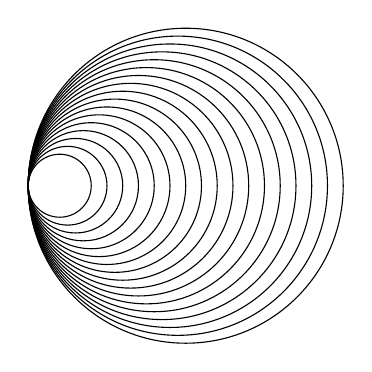
\begin{tikzpicture}[scale=0.1]
\foreach \n in {4,...,20}
	\draw (\n,0) circle (\n cm);
\end{tikzpicture}
}
\caption{Primeras $16$ iteraciones del pendiente hawaiiano.}
\end{marginfigure}

\begin{proposition}\labprop{CWProd}
El producto de CW-complejos finitos es un CW-complejo finito.
\end{proposition}

\begin{proof}
Sean $\mc{C}=\{D_i^k:\; k=0,1,\dots,n; \;i=1,2,\dots,r_k\}$ y $\mc{D}=
\{\Delta_\ell^j:\; j=0,1,\dots,m; \;\ell=1,2,\dots,r_j\}$ respectivas
descomposiciones celulares de $X$ e $Y$. Queremos ver que el conjunto
\[\mc{E}=\{U\times V: U\in \mc{C}, V\in \mc{D}\}\]
forma una descomposición celular de $X\times Y$.

Claramente, los elementos de $\mc{E}$ son disjuntos dos a dos por
construcción. Veamos que forman un recubrimiento de $X\times Y$: 
\[X\times Y=
	\left(\bigcup_{U \in \mc{C}} U\right)\times
	\left(\bigcup_{V \in \mc{D}} V\right)=
	\bigcup_{\substack{U \in \mc{C}\\V \in \mc{D}}} U\times V\]

Para demostrar este resultado, aplicaremos el \refthm{TCCWF}: dados
$i,j,k,\ell$,
\begin{align*}
U&=(\overline{D^k_i\times \Delta^\ell_j})\backslash
	(D^k_i\times \hat D^\ell_j)=
	(\overline{D^k_i}\times \overline{\Delta^\ell_j})\backslash
	(D^k_i\times \hat D^\ell_j)=\\
	&=[(\overline{D^k_i}\backslash D^k_i)\times \overline{\Delta^\ell_j}]\cup
	[\overline{D^k_i}\times (\overline{\Delta^\ell_j}\backslash \Delta^\ell_j)]
\end{align*}
Sabemos por hipótesis que $(\overline{D^k_i}\backslash D^k_i) \subseteq
X^{k-1}$ y $\overline{\Delta^\ell_j}\backslash \Delta^\ell_j \subseteq
Y^{\ell-1}$, por lo que $U \subseteq (X\times Y)^{k+\ell-1}$. Esto prueba la
primera condición.

Pasemos a la segunda: sean $U \in \mc{C}$ y $V \in \mc{D}$. Si
\begin{align*}
f\colon (D^k,S^{k-1}) \to (\overline{U},\overline{U}\backslash U); &&
g\colon (D^\ell,S^{\ell-1}) \to (\overline{V},\overline{V}\backslash V)
\end{align*}
son homeomorfismos relativos, se tiene que
\[f\times g\colon (D^{k+\ell},S^{k+\ell-1}) \to
(\overline{V\times V},(\overline{U\times V})\backslash (U\times V))\]
es un homeomorfismo relativo.
\end{proof}

\begin{example}\labexample{CWlindro}
\begin{enumerate}
\item El cilindro con bordes se define como $C=S^1\times [0,1]$. Podemos
asignar una estructura de CW-complejo a $C$ usando una estructura prefijada
de $S^1$ y otra de $[0,1]$:

\begin{align*}
[0,1]
\begin{cases}
\text{0-células:}	&p=\{0\}\\
					&q=\{1\}\\
\text{1-células:}	&\alpha=]0,1[
\end{cases}
&&
S^1
\begin{cases}
\text{0-células:}	&r=\{(1,0)\}\\
\text{1-células:}	&\beta=S^1-r
\end{cases}
\end{align*}

Estas estructuras inducen la siguiente descomposición celular sobre el cilindro:
\[C \begin{cases}
\text{0-células:}	&p\times r, q\times r\\
\text{1-células:}	&\alpha \times r, p\times \beta, q\times \beta\\
\text{2-células:}	&\alpha \times \beta
\end{cases}\]

\item El toro se puede expresar como $S^1\times S^1$, por lo que admite una
estructura de CW-complejo finito.

Consideremos la siguiente descomposición celular de $S^1$:
\begin{align*}
S^1
\begin{cases}
\text{0-células:}	&p=\{(1,0)\}\\
\text{1-células:}	&\alpha=S^1-p
\end{cases}
&&
S^1
\begin{cases}
\text{0-células:}	&r=\{(1,0)\}\\
\text{1-células:}	&\beta=S^1-r
\end{cases}
\end{align*}

Estas estructuras inducen la siguiente descomposición celular sobre el toro:
\[S^1\times S^1
\begin{cases}
\text{0-células:}&p\times r\\
\text{1-células:}&\alpha \times r,p\times \beta\\
\text{2-células:}&\alpha \times \beta
\end{cases}\]
\end{enumerate}
\end{example}

\begin{marginfigure}
\resizebox{\textwidth}{!}{
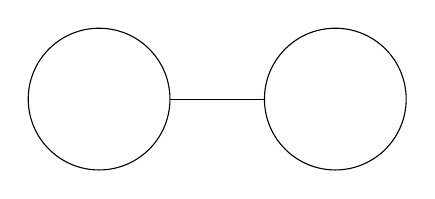
\begin{tikzpicture}
\draw (2,0) circle (.9cm);
\draw (1.1,0) -- (-.1,0);
\draw (-1,0) circle (.9cm);
\end{tikzpicture}
}
\caption[1-esqueleto del cilindro.]{1-esqueleto del cilindro. Observar que se
puede retraer en una figura ocho.}
\end{marginfigure}

\begin{marginfigure}
\includegraphics{Figures/ToroGeneradoresOrden1.pdf}
\caption{1-esqueleto del toro.}
\end{marginfigure}

\subsection{Subcomplejos}
Sea $X$ un CW-complejo finito y $\mc{C}$ una descomposición celular de $X$.
Decimos que un subespacio $A \subseteq X$ es un \textbf{subcomplejo} de $X$ si,
dado $D \in \mc{C}$, $D\cap A \neq \emptyset$ implica que $\overline{D}
\subseteq A$. Esta condición se puede expresar como que $A$ absorbe a todas
las células con las que entra en contacto.

Todo subcomplejo de un cierto complejo $X$ conforma un subespacio cerrado.
Además, aplicando el \refthm{TCCWF}, todo subcomplejo es un complejo en sí
mismo. En particular, todos los $k$-esqueletos de $X$ son subcomplejos.

\begin{proposition}
Si $A$ es un subcomplejo de un CW-complejo finito $X$, $A$ es un retracto por
deformación fuerte de algún entorno compacto de $A$ en $X$.
\end{proposition}

\begin{proof}
Sea $N$ el número de células que componen el espacio $X\backslash A$. Si
$N=0$, $X=A$, por lo que $A$ es un retracto por deformación fuerte de $X$ de
forma trivial y se sigue la tesis por compacidad de $X$.

Si $N=1$, existe una aplicación $f\colon S^{n-1} \to A$ continua tal que
$X=A\cup_f D^n$. En tal caso, podemos limitarnos a aplicar el
\reflemma{EntornoCompacto}.

Supongamos que el resultado es cierto para cualquier par de CW-complejos
finitos $(Y,B)$ tales que $Y\backslash B$ posee a lo sumo $N-1$ células, y sea
$(X,A)$ un par de CW-complejos tales que $X\backslash A$ tiene exactamente $N$
células. Si $D^m_i$ es una célula de $X\backslash A$ de dimensión máxima, se
define el subespacio $Y=X\backslash D^m_j$.

Queremos ver que $Y$ es un subcomplejo de $X$. Como $D^m_i$ es una célula de
dimensión máxima, todas las células de $X\backslash A$ tienen dimensión $m$ o
menos; de esta forma, toda célula de $X$ con dimensión mayor que $m$ forma
parte del subcomplejo $A$. En consecuencia, si $D^k_j$ es una célula de $Y$,
se tiene que $D^k_j \subset A$ ó $k \leq m$.

Si $D^k_j \subset A$, $\overline{D^k_j} \subseteq A$ por ser $A$ un
subcomplejo de $X$, de forma que
\[D^m_i \cap \p D^k_j \subseteq D^m_i \cap A=\emptyset\]
En cambio, si $k \leq m$, se tiene por \refthm{TCCWF} que
\[\p D^k_j=\overline{D^k_j}\backslash D^k_j\subseteq X^{k-1}\]
Dado que $k-1 < m$, se cumple una vez más que $D^m_i \cap \p D^k_j=\emptyset$.
Se sigue que $Y$ es subcomplejo de $X$.

Dado que $A$ es un subcomplejo de $X$ y $D^m_i \subset X\backslash A$, $A\cap
D^m_i=\emptyset$, por lo que es un subcomplejo de $Y$. Como $Y$ tiene una
célula menos que $X$, el par $(Y,A)$ verifica la hipótesis de inducción, por
lo que existe un entorno $U_1$ compacto de $A$ en $X$ tal que $A$ es un
retracto por deformación fuerte de $U_1$.

Sea $f\colon S^{m-1} \to Y$ una aplicación continua tal que $X=Y\cup_f D^m$.
Podemos hallar un homeomorfismo relativo
\[\phi\colon (D^m,S^{m-1}) \to
	(\overline{D^m_i}, \overline{D^m_i}\backslash D^m_i)\]
que extienda a $f$ de forma continua. Como $U_1$ es compacto en $Y$ y $\phi$
es un homeomorfismo, $\phi^{-1}(U_1)$ es un compacto de $S^{m-1} \subset D^m$.
Si
\begin{diag}
r\colon D^m\backslash\{0\} \arrow[r] & S^{m-1}\\[-8mm]
x \arrow[maps to,r]& \frac{x}{\|x\|}
\end{diag}
es la retracción radial, el conjunto
\[V=\{\phi(x): x \in D^m,\; \|x\| \geq 1/2,\; r(x) \in \phi^{-1}(U_1)\}\]
también es compacto.

Veamos cómo se construye el conjunto $V$: las células se adhieren al
CW-complejo por el borde, por lo que podemos pensar que la aplicación $\phi$
abomba $D^m$ para darle forma de hemisferio y pegarlo a $Y$ por la línea del
ecuador. Se tiene entonces que $X=Y\cup \phi(D^m)$ (ver \reffig{ECompacto1}).

Dado que $Y\cap \phi(D^m)=f(S^{m-1})$, $\phi^{-1}(U_1)=f^{-1}(U_1)$ está
contenido en $S^{m-1}$. En particular, $x$ no tiene por qué estar en
$\phi^{-1}(U_1)$, por lo que lo retraemos mediante una aplicación adicional.
Finalmente, elegimos sólo los puntos que están entre las esferas concéntricas
de radios $1/2$ y $1$ (ver \reffig{PhiMenos1V}).

El conjunto $U_1 \cap V$ es un retracto por deformación de $V$, y $A$ es un
retracto por deformación de $U_1$, de forma que $A$ será un retracto por
deformación de $U_1 \cup V$ (ver \reffig{ECompacto2}).

\begin{marginfigure}
\begin{subfigure}[b]{\textwidth}
\resizebox{\textwidth}{!}{
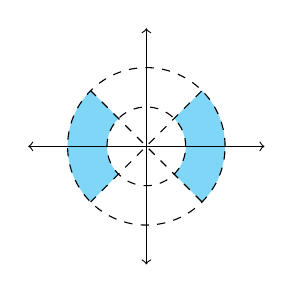
\begin{tikzpicture}

%Esta instrucción colorea arcos "gorditos" de circunferencia
\fill[cyan!50] (45:.5) arc[start angle=45, end angle=-45, radius=.5] -- (-45:1)
	arc[start angle=-45, end angle=45, radius=1] -- cycle;
\fill[cyan!50] (135:.5) arc[start angle=135, end angle=225, radius=.5] -- (225:1)
	arc[start angle=225, end angle=135, radius=1] -- cycle;


\draw[to-to] (1.5,0) -- (-1.5,0);
\draw[to-to] (0,1.5) -- (0,-1.5);

\draw[dashed] (0,0) circle (1 cm) circle (.5 cm);

%Scope y clip cortarán las rectas donde se acaben las circunferencias
\clip (0,0) circle (1 cm);
\draw[dashed] (1,1) -- (-1,-1);
\draw[dashed] (1,-1) -- (-1,1);


\end{tikzpicture}
}
\caption{\labfig{PhiMenos1V} El conjunto $\phi^{-1}(V)$ corresponde a la
región coloreada. $\phi^{-1}(U_1)$ son los puntos de la región coloreada que
recaen sobre la esfera de radio $1$.}
\end{subfigure}
\begin{subfigure}[b]{\textwidth}
\resizebox{\textwidth}{!}{
\begin{tikzpicture}

\draw[dashed, fill=cyan!50] (1.5,2) circle (1cm);

\begin{scope}
\clip 	(0,0) .. controls (1,-1) and (2,-1) ..
		(3,0) .. controls (4,1) and (2,2) ..
		(3,4) .. controls (2,4) and (1,3) ..
		(0,4) .. controls (-1,3) and (1,2) ..
		(0,0);

\draw[pattern=north east lines]
	(0,1.5) .. controls (1,3.5) and (2,1.5) .. (4,4.5) --
	(4,4) .. controls (2,1) and (1,3) .. (0,1);

\draw[very thick] (4,4) .. controls (2,1) and (1,3) .. (0,1);
	
\draw[pattern=north east lines]
	(4,4) .. controls (2,1) and (1,3) .. (0,1) --
	(0,.5) .. controls (1,2.5) and (2,.5) .. (4,3.5);
\end{scope}

\draw (3.25,2.75) node {$A$};
\draw (0,1) -- (-.2,1) -- (-.2,2) -- (0,2);
\draw (-.6,1.5) node {$U_1$};

\draw 	(0,0) .. controls (1,-1) and (2,-1) ..
		(3,0) .. controls (4,1) and (2,2) ..
		(3,4) .. controls (2,4) and (1,3) ..
		(0,4) .. controls (-1,3) and (1,2) ..
		(0,0);

\end{tikzpicture}
}
\caption{Representación de los conjuntos $A$, $U_1$ y la bola $\phi(D^m)$ en
	$Y$.}
\end{subfigure}
\begin{subfigure}[b]{\textwidth}
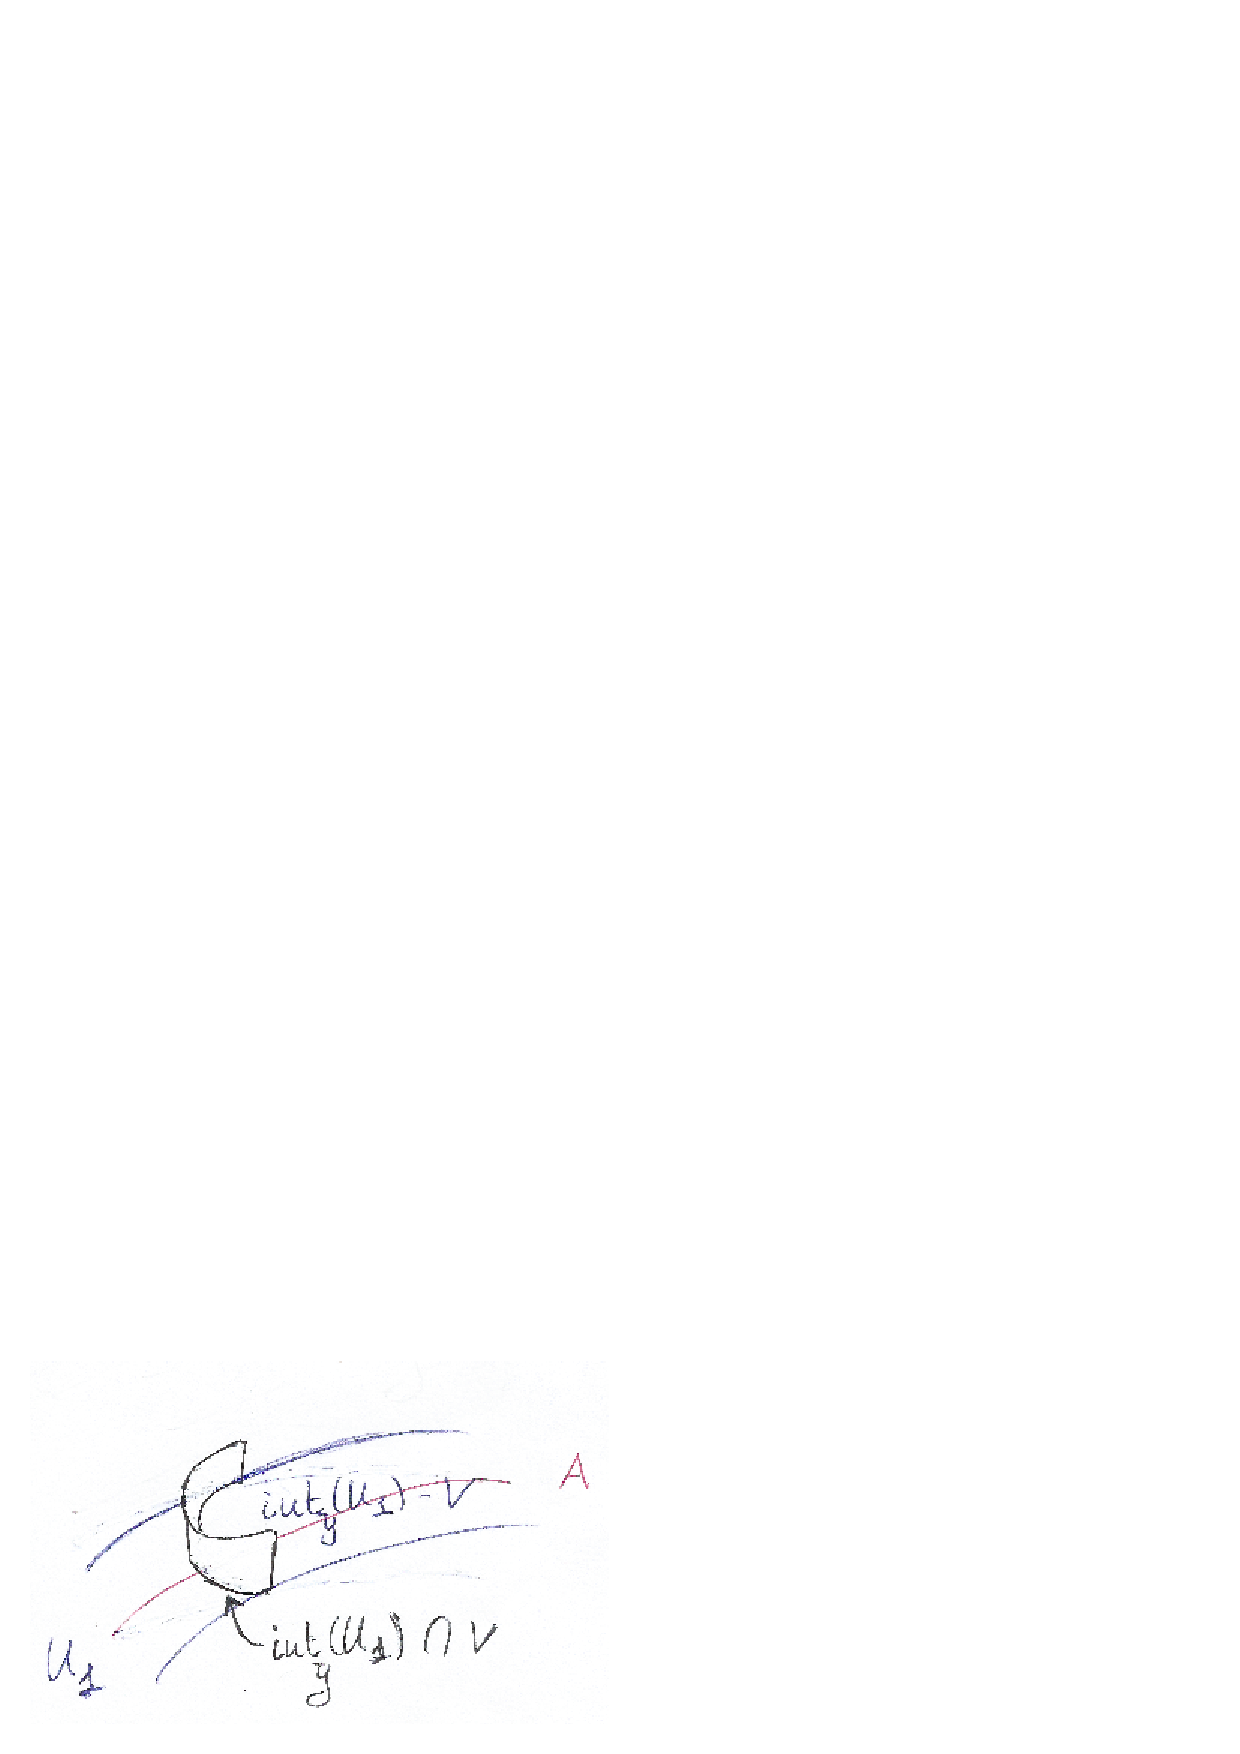
\includegraphics{Figures/ECompacto2.pdf}
\caption{\labfig{ECompacto2} Podemos retraer $V$ (superficies arqueadas) en
$U_1$ (banda plana) y $U_1$ en $A$ (línea discontinua).}
\end{subfigure}
\caption{Pasos ilustrados de la demostración.}
\end{marginfigure}

Ya sabemos que $U_1 \cup V$ se puede retraer en $A$. Dado que es unión de
compactos, es trivialmente compacto, de forma que habremos terminado la
demostración si podemos probar que $U_1 \cup V$ es entorno en $X$ de $A$.

Sea $y \in \Int_Y(U_1)$. Si $y \not\in V$, $y \in \Int_X(U_1)$
(repersentado como una banda en la ilustración \ref{ECompacto2}), por lo que
también estará en $\Int_X(U_1 \cup V)$.

Si $y \in V$, se tiene que $y \in \overline{D^m_i}\backslash D^m_i=
\phi(D^m\backslash \p D^m)=f(S^{m-1})$. Por otro lado,
$\phi^{-1}(\Int_Y(U_1))$ es un abierto de $S^{m-1}$ que contiene a
$\phi^{-1}(y)$ (por cómo se define $V$), de forma que 
\[\phi^{-1}(y) \in \Int_{S^{m-1}}\phi^{-1}(V) \implies y \in
\Int_{\overline{D^m_i}}(V)\]
Dado que $D^m_i$ es una célula de $X$, se sigue que $y \in
\Int_X(U_1\cup V)$.

Como $U_1$ es un entorno de $A$ en $Y$,
\[A \subseteq \Int_Y(U_1)\subseteq \Int_X(U_1\cup V)\]
por lo que $U_1\cup V$ es entorno de $A$ en $X$. Pero eso es lo que nos
quedaba por demostrar.
\end{proof}

\section{Grupos de homología celular}
\begin{corollary}\label{HomoCelular}
Si $X$ es un CW-complejo finito y $X^k$ es el $k$-esqueleto de $X$,
\[H_j(X^k,X^{k-1})=0 \quad \forall j \neq k\]
Además, $H_k(X^k,X^{k-1})$ es un grupo abeliano libre con un generador por
cada $k$-célula de $X$, conocido como el \textbf{grupo de homología celular}
de orden $k$.
\end{corollary}

\begin{proof}
Sabemos que $X^{k-1}$ es un subcomplejo de $X^k$. Por la proposición anterior,
existe un entorno compacto $U \subseteq X^k$ de $X^{k-1}$ tal que $X^{k-1}$
es un retracto por deformación fuerte de $U$.

Como $X$ es un CW-complejo finito, podemos hallar un homeomorfismo relativo
\[\phi: (\mc{D}^k, \mc{S}^{k-1}) \longrightarrow (X^k,X^{k-1})\]
utilizando los homeomorfismos $h$ que nos proporciona el teorema de
caracterización de CW-complejos finitos. Aplicando el teorema del
homeomorfismo relativo, se sigue que 
\begin{align*}
H_*(X^k,X^{k-1}) &\cong H_*(\mc{D}^k,\mc{S}^{k-1}) \cong 
	\sum^r_{i=1} H_*(D_i^k, S_i^{k-1}) \\
	& \cong \sum^r_{i=1} \tilde{H}_*(S^k) \cong
	\tilde{H}_*(S^k)^r \cong
	\begin{cases}
	\mb{Z}^r&\text{ si }p=k\\
	0&\text{ si no}
	\end{cases}
\end{align*}
\end{proof}

\begin{example}
Vamos a calcular la homología de la rosa de $p$ pétalos utilizando los grupos
de homología celular. Por la proposición \refprop{HomoCW},
\[H_j(B_p)\cong H_j(\{\star\})=0\]
para todo $j > 1$. Para $j=1$,
\[H_1(B_p)\cong \tilde{H}_1(B_p)\cong H_1(B_p,\{\star\})\]
Dado que $\{\star\}$ es el $0$-esqueleto de $B_p$, que tiene $p$ $1$-células, se
tiene que dicho grupo es isomorfo a $\mb{Z}^p$.
\end{example}

\section{Homología de la $n$-rosa}
Para $j=1,\dots,p$, sea $f_j\colon \p D^n \to \{\star\}$ la aplicación
constante. Se define la $n$-rosa de $p$ pétalos como la adjunción
\[X=B^n_p=\{\star\}_{f_1,\dots,f_p}\]

Por el corolario \ref{HomoCelular}, sabemos que $H_n(X^n,X^{n-1})\cong 
\mb{Z}^p$ y\\ $H_m(X^n,X^{n-1})=0$ para todo $m\neq n,0$. Sin embargo, $X^{n-1}
=X^0=\{\star\}$, por lo que
\begin{align*}
\mb{Z}^p\cong H_n(X,X^{n-1})=\tilde H_n(X);\\
0=H_m(X,X^{n-1})=\tilde H_m(X); && (m\neq n)
\end{align*}

\begin{theorem}\labthm{nrosa}
\[\tilde H_m(B^n_p)\cong
\begin{cases}
\mb{Z}^p & \text{si $m=n$}\\
0 & \text{si $m\neq n$}
\end{cases}\]
\end{theorem}

Al igual que pasaba con la $1$-rosa, cada pétalo que adjuntamos aporta un nuevo
generador, sólo que en este caso es la clase de un $n$-símplice singular.

\subsection{Rosa mixta}
¿Qué pasaría si mezcláramos pétalos de diferentes dimensiones? Intuitivamente,
cada pétalo de dimensión $k$ debería añadir un generador de orden $k$.

Sea $\alpha=(\alpha_1,\dots,\alpha_n) \in \mb{N}^n$. Si $f\colon \{\star\} \to
\{\star\}$ es la identidad, definimos
\[B_\alpha:=\{\star\}\cup_f B^1_{\alpha_1}\cup_f B^2_{\alpha_2}\cup_f \dots
\cup_f B^n_{\alpha_n}\]
siendo $B^k_0=\{\star\}$.

\begin{marginfigure}
\includegraphics{Figures/B22.png}
\caption{Ejemplo de rosa mixta $B_{(2,2)}$.}
\end{marginfigure}

\begin{theorem}\footnote{Este resultado está basado en una conversación que
tuve con mi directora del TFG, pero no pensé en añadirlo en su momento.}
\labthm{RosaMixta}
Dado $\alpha \in \mb{N}^n$,
\[H_m(B_\alpha)\cong
\begin{cases}
\mb{Z}			& \text{si $m=0$}\\
\mb{Z}^{\alpha_i} 	& \text{si $m=i$}\\
0				& \text{si $m > n$}
\end{cases}\]
\end{theorem}

\marginnote[-2.2cm]{
\begin{kaobox}[frametitle=Idea de la demostración]
\begin{itemize}
\item Probamos que la tesis se cumple cuando la rosa tiene $k_1$ pétalos de
dimensión $1$ (ya lo hemos hecho).
\item Suponemos que la tesis se cumple cuando la rosa tiene $k_1$ pétalos de
dimensión $1$, $k_2$ pétalos de dimensión $2$, y así hasta dimensión $n-1$.
\item Probamos que, como consecuencia, la tesis se cumple cuando añadimos $k_n$
pétalos de dimensión $n$.
\end{itemize}

Esta prueba puede ser conceptualmente engorrosa, así que es recomendable tratar
de hacer primero ejemplos para $n=2,3,4$.
\end{kaobox}
}

\begin{proof}
Si $\alpha=(\alpha_1,\dots,\alpha_n)$, procedemos por inducción sobre $n$. Si
$n=1$, $B_\alpha$ es una $1$-rosa de $\alpha_1$ pétalos, y la tesis se cumple
por \refthm{nrosa}.

Sea $\alpha'=(\alpha_1,\dots,\alpha_{n-1})$, y $X=B_{\alpha'}$. Supongamos que
la tesis se cumple para $X$ y sean $f_i\colon S^{n-1} \longrightarrow \{\star\}$
aplicaciones constantes. Tenemos entonces que
\[B_\alpha=X_{f_1\dots f_{\alpha_n}}\]

Por la \refprop{HomoCW}, si $(f_i)_*\colon \tilde H_{n-1}(S^{n-1})\to
H_{n-1}(\{\star\})=\{0\}$, se cumple lo siguiente:
\begin{enumerate}
\item Para todo $p\neq n,n-1$,
\[H_p(X_{f_1\dots f_{\alpha_n}})=H_p(X)\]
Por hipótesis de inducción, $H_p(X)\cong \mb{Z}^{\alpha_p}$ cuando $p < n-1$ y
$\{0\}$ cuando $p > n-1$.
\item Como $(f_i)_*$ va a parar a $\{0\}$ para todo $i$, $\im (f_i)_*=\{0\}$ y
\begin{align*}
H_{n-1}(X_{f_1\dots f_{\alpha_n}})&\cong
	\frac{H_{n-1}(X_{f_1\dots f_{\alpha_n-1}})}{\im (f_{\alpha_n})_*}\cong
	H_{n-1}(X_{f_1\dots f_{\alpha_n-1}})\cong\\
	&\cong \frac{H_{n-1}(X_{f_1\dots f_{\alpha_n-2}})}{\im (f_{\alpha_n-1})_*}\cong
	H_{n-1}(X_{f_1\dots f_{\alpha_n-2}})\cong\\
	&\cong \dots \cong H_{n-1}(X)
\end{align*}
Por hipótesis de inducción una vez más, ésto es $\mb{Z}^{\alpha_{n-1}}$.
\end{enumerate}

El tercer ítem requiere que hagamos inducción sobre el número de pétalos de
dimensión $n$\footnote{Al principio, pensé que era necesario tratar este
resultado como una \emph{doble inducción}, así que decidí leer sobre el tema.
Si bien he conseguido reducirlo a una inducción aislada dentro de otra, creo
que es un tema interesante, así que he decidido escribir un pequeño apéndice
sobre el tema.}. Dado un espacio $Y$ arbitrario, sabemos por la
\refprop{HomoCW} que la secuencia
\[0 \longrightarrow H_n(Y) \longrightarrow H_n(Y_{f})
\longrightarrow \ker f_*\longrightarrow 0\]
es exacta. En particular, $\ker f_*=\tilde H_{n-1}(S^{n-1})\cong \mb{Z}$ por el
\labthm{HRelSn}, por lo que
\begin{equation}
\mb{Z}\cong \frac{H_n(Y_f)}{H_n(Y)} \label{ExactaZ}
\end{equation}
En este caso, $H_n(X)=\{0\}$ por hipótesis de inducción, por lo que
$H_n(X_{f_1})\cong \mb{Z}$.

Supongamos que $H_n(X_{f_1\dots f_{\alpha_n-1}})\cong \mb{Z}^{\alpha_n-1}$.
Usando \eqref{ExactaZ}, concluimos que
\[H_n(X_{f_1\dots f_{\alpha_n}})\cong H_n(X_{f_1\dots f_{\alpha_n-1}})\oplus
\mb{Z}\cong \mb{Z}^{\alpha_n}\]
concluyendo así ambas inducciones. Se sigue la tesis.
\end{proof}
